\documentclass{article}
\usepackage[utf8]{inputenc}
\usepackage{amsmath}
\usepackage{amssymb}
\usepackage{graphicx}
\usepackage[margin = 1 in]{geometry}
\usepackage{algorithm}
\usepackage{algpseudocode}
\usepackage{booktabs}
\usepackage{verbatim}
%\usepackage{indentfirst}

\title{CS5220 Project 2: Shallow Water Equations}
\author{Nick Cebry, Jiahao Li, Max Ruth}
\date{October 5, 2020}

\begin{document}

\maketitle

\section{Introduction}

In this project, we worked with the a finite volume solver for the shallow water equations. These PDEs model the movement of waves in scenarios where the waves are long compared to the depth of the water. We were provided with a moderately performant single threaded version of the code, and made an effort to improve performance by parallelizing the algorithm. For our implementation, we chose to use MPI as our parallelization paradigm. Our algorithm divides the grid up into a series of subdomains, and assigns one subdomain to each processor. Processors are responsible for calculating the behavior of the water in their portion of the domain. They communicate information about the cells on the edge of their domain with the processors of neighboring domains so that information propagates properly across domain boundaries.

The aims for this project are: 1) using MPI as parallelization implementation for the single-core code; 2) conducting weak and strong scaling studies on the shallow water problem to test the robustness of our implementation; 3) profiling and tuning the codes for higher-level optimization based on computational resources.

\section{The Algorithm}
\textbf{For the purposes of this algorithm, we are considering two consecutive calls to \texttt{central2d\_step} to be ``one time step,'' in order to alleviate any confusion with the shifting grids in Jiang and Tadmor.}

To address the problem of parallelizing the method of Jiang and Tadmor, we use a domain decomposition method like the one introduced for Conway's Game of Life. For the problem, we assume that the domain $\Omega = (0,L)^2$ is divided into square cells, with a resolution of $M$ cells in each direction. Because the problem is periodic, this amounts to $M$ ``points'' at which the height $h$, $x$-velocity $u$, and $y$-velocity $v$ are known. To parallelize the code, we divide the domain into an $N_x\times N_y$ grid of subdomains, where each subdomain is owned by a process. By this construction, we are using a total of $N_x N_y$ processors. 

As a part of this construction, each subdomain is responsible for knowing the value of $m_x \times m_y$ points \textit{at all times} where $m_x = M/N_x$ and $m_y = M/N_y$. However, due to the way information flows through a hyperbolic system of equations, we also require each processor to store a ``halo'' of ghost cells with width $m_g.$ Each processor is not tasked with knowing the value of the ghost cells, but rather retrieves the values of the ghost cells from its neighbors. The width of the halo is related to how many time steps each processor can perform independently before information must be exchanged -- called $m_t$ -- by the relation $m_g = 4 m_t$. Independent of the number of processors (assuming $M$ is fixed), the we will call the total number of time step blocks $N_t$, so that the total number of time steps is $m_t N_t$. 

We must also keep track of the maximum speed of information across all of the processors, so that each processor takes the same time step. In the code, we are currently sharing this information \textit{at every time step}, but this turns out not to be a large burden for the sizes of problems we are considering. 

In total, the algorithm can be summarized by Alg.~\ref{alg:PJT}. Inside of the main loop, we first share the ghost cells. This goes in the order of pass-left and receive-right; pass-right and receive-left; pass-up and receive-down; pass-down and receive-up. In the left/right passing of ghost cells, we pass a block of size $m_g m_y$, whereas for up/down we pass a block of size $m_g (m_x + 2m_g)$, as we need to communicate the corners of the halo along with the sides in this step. 
\begin{algorithm}
\caption{Parallel Jiang-Tadmor Main Loop}\label{alg:PJT}
\begin{algorithmic}
\For {$i \gets 1$ to $N_t$}
    \State Share ghost cells via 4 calls of \texttt{MPI\_Sendrecv}
    \For{$j \gets 1$ to $m_t$}
        \State Get local time step using \texttt{speed}
        \State Get global time step via \texttt{MPI\_Allreduce}
        \State Perform time step
    \EndFor
\EndFor
\end{algorithmic}
\end{algorithm}

\subsection{Model Speed Up}



The general process:
\begin{enumerate}
	\item Used MPI
	\item Transfer Boundary information to left and right neighbors, the top and bottom (transferring the corners to top and bottom)
	\item Transfer boundary information every $\tau$ steps
	\item Transfer time step information every $\tau$ steps as well (This is what is being used in the model anyway)
\end{enumerate}
The model
\begin{enumerate}
	\item Four different contributions to batches of time steps
	\item Give predictions for how strong scaling, weak scaling, and optimal time batching look like.
\end{enumerate}

\section{Scaling and Profiling Results}
\subsection{Scaling Studies}
We performed both strong and weak scaling studies to analyze the
performance of our algorithm. For the strong scaling study, we used the
dam break scenario, and fixed the resolution of the grid cells at 1000
cells in both the X and Y dimensions. We then varied the number of
processors used to compute the simulation up until a fixed simulation
time. The size of the sub-domains varied with the number of processors in
order to keep the problem size constant. We compare the wall clock time
required to solve a fixed problem as the amount of compute resources
available varies. For the weak scaling study, we again used the dam break
scenario, but varied the resolution of the grid cells with the number of
processors used. The resolution of the grid was varied such that each sub-
domain was always 300 cells on each side. The simulation was run until a
fixed amount of time had been simulated. In order to account for the
different CFL conditions with different grid resolutions, we recorded the
total number of time steps processed, and divided the wall clock time by
this number to determine the average amount of time required to compute a
single tick of the simulation. We compare the wall clock time required to
compute a single simulation tick as both the size of the problem and the
computational resources available scale. Additionally, for both types of
scaling tests we analyzed the impact of varying the frequency of
communication between sub-domains. These tests explored the tradeoff
between frequency of suffering the penalty of communication and amount
of data communicated and duplicated computation performed.

\begin{table}
\resizebox{\textwidth}{!}{
\begin{tabular}{cccccccccc}
  \toprule
  sub-domain grid & nproc & \multicolumn{8}{c}{simulation ticks per communication} \\\cmidrule(r){3-10}
                  &                 & 1 & 2 & 3 & 4 & 5 & 6 & 7 & 8 \\\midrule
  1x1 &  1 & 138.95 & 140.02 & 136.78 & 130.53 & 119.90 & 130.60 & 160.26 & 171.99 \\\midrule
  2x2 &  4 &  48.23 &  48.17 &  48.62 &  29.87 &  47.93 &  51.60 &  30.35 &  51.15 \\\midrule
  3x3 &  9 &  30.36 &  30.65 &  32.47 &  34.00 &  30.08 &  35.37 &  32.00 &  39.20 \\\midrule
  4x4 & 16 &   9.50 &  10.78 &  12.11 &  13.88 &  14.88 &  17.04 &  16.48 &  20.62 \\\midrule
  5x5 & 25 &   3.76 &   3.72 &   3.89 &   4.41 &   4.63 &   6.23 &   6.52 &   8.85 \\\midrule
  6x6 & 36 &   2.69 &   2.62 &   2.65 &   2.76 &   2.81 &   3.08 &   2.99 &   3.67 \\\midrule
  7x7 & 49 &   2.22 &   2.07 &   2.13 &   2.17 &   2.20 &   2.39 &   2.30 &   2.70 \\\midrule
  8x8 & 64 &   1.92 &   1.72 &   1.73 &   1.83 &   1.83 &   2.05 &   1.88 &   2.32 \\\midrule
  9x9 & 81 &   1.62 &   1.46 &   1.41 &   1.51 &   1.53 &   1.78 &   1.56 &   1.89 \\\bottomrule
\end{tabular}
}
\caption{Strong scaling study data}
\label{table:strong}
\end{table}

\begin{figure}
\centering
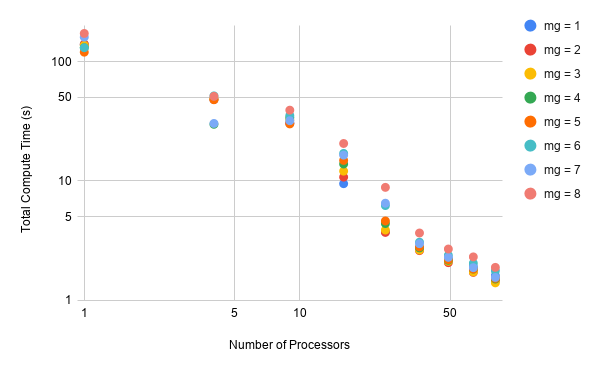
\includegraphics[width=0.75\textwidth]{strong.png}
\caption{Strong scaling study performance}
\label{fig:strong}
\end{figure}

The data collected from the strong scaling test is shown in
Table \ref{table:strong}. The data in this table is the wall clock time
required for the computation. We see the processing time decrease as the
number of processors increases. We have also presented this data in
graphical form in Figure \ref{fig:strong}.

\begin{table}
\resizebox{\textwidth}{!}{
\begin{tabular}{cccccccccc}
  \toprule
  sub-domain grid & nproc & \multicolumn{8}{c}{simulation ticks per communication} \\\cmidrule(r){3-10}
                  &                 & 1 & 2 & 3 & 4 & 5 & 6 & 7 & 8 \\\midrule
  1x1 &  1 & 5.33e4 & 3.47e4 & 3.57e4 & 4.87e4 & 3.88e4 & 4.19e4 & 2.99e4 & 2.59e4 \\\midrule
  2x2 &  4 & 6.22e4 & 4.04e4 & 3.93e4 & 4.20e4 & 3.59e4 & 3.53e4 & 2.92e4 & 6.26e4 \\\midrule
  3x3 &  9 & 3.96e4 & 4.12e4 & 3.72e4 & 3.64e4 & 3.67e4 & 3.55e4 & 3.27e4 & 3.88e4 \\\midrule
  4x4 & 16 & 5.45e4 & 5.21e4 & 5.04e4 & 4.62e4 & 4.92e4 & 4.84e4 & 4.04e4 & 4.37e4 \\\midrule
  5x5 & 25 & 6.79e4 & 6.44e4 & 6.10e4 & 5.89e4 & 5.48e4 & 5.51e4 & 5.00e4 & 5.15e4 \\\midrule
  6x6 & 36 & 8.03e4 & 7.62e4 & 7.32e4 & 7.13e4 & 6.82e4 & 6.23e4 & 5.98e4 & 5.85e4 \\\midrule
  7x7 & 49 & 9.38e4 & 8.82e4 & 8.49e4 & 8.17e4 & 7.67e4 & 7.35e4 & 6.97e4 & 6.67e4 \\\midrule
  8x8 & 64 & 1.02e5 & 9.59e4 & 9.38e4 & 8.99e4 & 8.63e4 & 8.32e4 & 7.82e4 & 7.45e4 \\\midrule
  9x9 & 81 & 1.16e5 & 1.11e5 & 1.05e5 & 9.98e4 & 9.69e4 & 9.43e4 & 8.77e4 & 8.39e4 \\\bottomrule
\end{tabular}
}
\caption{Weak scaling study data}
\label{table:weak}
\end{table}

\begin{figure}
\centering
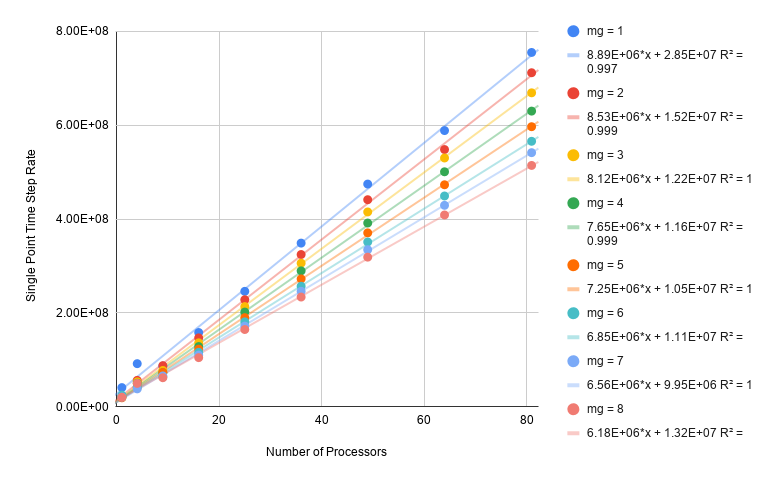
\includegraphics[width=0.75\textwidth]{weak.png}
\caption{Weak scaling study performance}
\label{fig:weak}
\end{figure}

For the weak scaling study, we collected data on the amount of work
accomplished per time. To get this number, we multiplied the number of
cells in the simulation by the number of time steps computed, and divided
by the wall clock time. This data is presented in Table \ref{table:weak}.
As expected, the size of the problem we can compute in a given amount of
time increases as the number of processors increase. We present a graph of
this data in Figre \ref{fig:weak}.

\subsection{Profiling}

We used Tau package on Comet as the profiler tool to study the performance of our parallelization and higher-level optimization of the original codes. We used compiler-based instrumentation method, which records timing for both the MPI routines and user-defined functions in the codes. By changing the compiler from \texttt{mpicc} to \texttt{tau\_cc.sh} and adding \texttt{-tau\_options=-optCompInst} to the argument for compiling, running the program returns profiling results for each processor and we can look them up by \texttt{pprof} command. The profiling result shows the proportion of time spent, exclusive time, the total inclusive time, number of calls, number of subroutines as well as the average inclusive time per call for each of the functions in the program. As the parallel computing on each individual processor, except for the rank $0$ core where we expect to see different behavior due to all the subdomain data gathering to output solution after certain time steps for a rationale check, mostly the mean times spent on all the cores are compared straightforward. 

We first did a direct profiling comparison between a $200\times200$ grid and a $1000\times1000$ grid, where in both cases 9 processors (blocking into $3\times3$) were called based on Comet terminal environment. Since the two are computed using the same number of cores, the main difference is the size of subdomains divided into each core, which also indicates blocking size affects the performance of codes. For a small grid problem, the \texttt{MPI\_Init()} used $35.5\%$ of the total profiling time; the major of the code \texttt{central2d\_xrun} consists of three parts, \texttt{central2d\_step}, \texttt{central2d\_periodic} and a MPI routine \texttt{MPI\_Allreduce()}, taking up $53.0\%$, $7.0\%$ and $0.0\%$, respectively. \texttt{central2d\_periodic} is the modified code for inter-core communication of ghost cell; \texttt{MPI\_Allreduce()} is used for synchronizing each subdomain at the same physical time. Numerical PDE computing as well as core communication does not take up fully.  When using same amount of computational resources, the situation of the large scale becomes different, where  \texttt{central2d\_step}, \texttt{central2d\_periodic} and  \texttt{MPI\_Allreduce()} take up $95.1\%$, $3.3\%$ and $0.0\%$ of the total time; \texttt{MPI\_Init()}  is only $0.1\%$. This indicates the bottleneck in a large scale problem running on 9 processors is positioned on how to make the PDE computing itself faster. The most time is spent on the actual PDE numerical computing, whereas the cost of core communication is pretty low. The profiling tables are attached at the end of the report.

\subsection{Tuning with Blocking}

So a direct way to speed up the computation in the large-scale problem is to introduce more resources, i.e. to decompose into more blocks and assign to more processors. We used \texttt{sbatch} command on both Graphite and Comet to submit the task in order to take advantage of the huge computational resources on these two large-scale server. A code profiling was also run by Tau on Comet utilizing 81 cores (blocking into $9\times9$), for comparison with the one using only 9 cores. Under this circumstance, the total time spent on running the whole program with profile instrumentation is greatly reduced, from 15min to 2min. When looking into the computing as well as communication, \texttt{central2d\_step}, \texttt{central2d\_periodic} and  \texttt{MPI\_Allreduce()} use up $69.3\%$, $6.0\%$ and $15.0\%$, respectively. It demonstrates that when deploying more cores to compute, the proportion of computing itself goes down, while communication and synchronization among each cores goes up. Compared with the small-scale, where the blocking size in each core is more comparable, the PDE computing is in the same scale but $9\times9$ consumes more average inclusive time per call since it still uses nearly twice as large the block size; same as the communication where $9\times9$ is around twice average per call since there are more data to exchange in the same amount of neighboring. The same trends can be found when compared with $3\times3$ on the same large-scale. However, more decomposition gives more distributed tasks to be done, meaning when the communication and synchronization is needed, it will pay more. Luckily, our parallelization optimizes the way of communication so that only the ghost cells have to be updated from the left, right, top and bottom neighboring blocks. Nevertheless, the cost of synchronization, as of \texttt{MPI\_Allreduce()}, grows tremendously from 22usec/call in $3\times3$ to 18823usec/call in $9\times9$. The blocking strategy is constraint to how many computational resources are available. There is also trade-off between the individual computing and synchronization. Block size also plays a key role in utilizing the cache. In our test, blocking works prominently well in large-scale study.

\subsection{Tuning with Time-step Batching}

After making the parallelized code speedup by having more individual processors, another way we tried on is to advance the time-step. In the original code, the iteration is based on a two-time-step staggered grids. During each iteration, the time is forwards two step to an updated status. In our primary parallelization, this means after two time-step, the periodic condition or individual core communication is needed in the area of the ghost cells. As a way to possible speedup, we can move forwards from the two time-step to more, so that the numbers of communication among each cores can be reduced, herein called time-step batching. We did a profile on the large-scale problem with $9\times9$ cores and a four time-step batching. The numbers of call of \texttt{central2d\_periodic} is reduced half, as expected half less of communication in four time-step batching; the inclusive total time is also decreased from 9164msec to 7437msec. However, since more time-step is forwards, which is proportional to the increase of numbers of ghost cells, as indicated that the average inclusive time per call is increased from 7562usec/call to 12437usec/call. At the same time, due to the demand of time-step synchronization, $dt$ has to be communicated in every time-step. So this time-step batching does not help much with the timing of \texttt{MPI\_Allreduce()} under this $9\times9$ 4 time-step batching setting. The time-step batching plays the trade-off between the numbers and the amount of required communication. However, we did not see much improvement in the implementation of large-scale study.



\section{Conclusion}
What we would add for next time:
\begin{enumerate}
	\item More careful cache performance
	\item Tuning number of ghost cells to block size
	\item Different sized domains/initial conditions
	\item Deal with the fact that not all processors are the same
	\item Think about the tradeoff between a conservative time step and communicating every step (how uneven are the time steps really?)
	\item Communication between processors at different nodes is different than that of the same nodes?
\end{enumerate}

\appendix
\section{Profiling table: small scale on 9 cores}
\noindent
{\footnotesize
\begin{verbatim}
FUNCTION SUMMARY (mean):
---------------------------------------------------------------------------------------
%Time    Exclusive    Inclusive       #Call      #Subrs  Inclusive Name
              msec   total msec                          usec/call 
---------------------------------------------------------------------------------------
100.0            6       16,162           1           1   16162524 .TAU application
100.0        0.954       16,156           1           3   16156274 main 
 63.8        0.596       10,313           1     119.444   10313260 run_sim 
 60.0       0.0372        9,703          50          50     194062 central2d_run 
 60.0        0.538        9,703          50        1250     194061 central2d_xrun 
 53.0            7        8,559         500     37833.3      17118 central2d_step 
 35.5        5,737        5,737           1           0    5737190 MPI_Init() 
 26.7           49        4,322         500      218000       8644 central2d_predict 
 26.0        4,175        4,205      213500     50014.3         20 limited_deriv1 
 26.0           68        4,200         500      309001       8401 central2d_correct 
 25.9        4,150        4,179      213500     49986.7         20 limited_derivk 
  7.0            1        1,135         250        7000       4542 central2d_periodic 
  7.0        1,131        1,131        1000           0       1131 MPI_Sendrecv() 
  3.0       0.0558          482          51     96.3333       9452 gather_sol 
  2.5        0.037          398     45.3333     45.3333       8787 send_full_u 
  2.5          398          398     45.3333           0       8787 MPI_Send() 
  0.6          104          104           1           0     104869 MPI_Finalize() 
  0.5           80           81          51     9614.89       1597 copy_u 
  0.5       0.0621           73     45.3333     90.6667       1631 recv_full_u 
  0.4           60           60     5.66667           0      10762 solution_check 
  0.4           43           58      100001      100001          1 limdiff [THROTTLED]
  0.2           12           28     36833.3     36833.3          1 shallow2d_flux 
  0.2           25           25     5.66667           0       4555 viz_frame 
  0.2           25           25           1           0      25248 MPI_Barrier() 
  0.1           20           20      100001           0          0 central2d_correct_sd [THROTTLED]
  0.1           16           16     36833.3           0          0 shallow2dv_flux 
  0.1           15           15      100001           0          0 xmin2s [THROTTLED]
  0.0            7            7    0.111111           0      66771 viz_close 
  0.0            5            5         250           0         22 MPI_Allreduce() 
  0.0            3            5           1     13333.3       5336 lua_init_sim 
  0.0            2            2        6000           0          0 copy_subgrid 
  0.0            2            2           1           0       2708 viz_open 
  0.0        0.133            2         250         250         10 shallow2d_speed 
  0.0            2            2         250           0          9 shallow2dv_speed 
  0.0            2            2     45.3333           0         47 MPI_Recv() 
  0.0            1            1       11837           0          0 central2d_offset 
  0.0            1            1     11111.2           0          0 central2d_offset [THROTTLED]
  0.0       0.0189       0.0201           1           2         20 central2d_init 
  0.0      0.00733      0.00733           1           0          7 copy_basic_info 
  0.0      0.00122      0.00122           2           0          1 central2d_free 
  0.0     0.000778     0.000778           1           0          1 MPI_Comm_size() 
  0.0     0.000444     0.000444           1           0          0 MPI_Comm_rank() 
\end{verbatim}
}

\section{Profiling table: large scale on 9 cores}
\noindent
{\footnotesize
\begin{verbatim}
FUNCTION SUMMARY (mean):
---------------------------------------------------------------------------------------
%Time    Exclusive    Inclusive       #Call      #Subrs  Inclusive Name
              msec   total msec                          usec/call 
---------------------------------------------------------------------------------------
100.0            5    15:34.549           1           1  934549844 .TAU application
100.0        0.461    15:34.543           1           3  934543980 main 
 99.8        0.763    15:32.687           1     119.444  932687449 run_sim 
 98.4       0.0854    15:19.270          50          50   18385400 central2d_run 
 98.4            4    15:19.269          50        6060   18385398 central2d_xrun 
 95.1        2,382    14:48.441        2424      104849     366519 central2d_step 
 47.7        1,531     7:25.437        2424 4.93526E+06     183761 central2d_predict 
 47.3     7:21.737     7:21.766 4.91345E+06       49979         90 limited_derivk 
 47.1        2,236     7:20.259        2424 4.99163E+06     181625 central2d_correct 
 47.1     7:20.090     7:20.119 4.91345E+06       50022         90 limited_deriv1 
  3.3            9       30,591        1212       33936      25240 central2d_periodic 
  3.3       30,494       30,494        4848           0       6290 MPI_Sendrecv() 
  1.1        0.131       10,712          51     96.3333     210043 gather_sol 
  0.9        0.102        8,610     45.3333     45.3333     189947 send_full_u 
  0.9        8,610        8,610     45.3333           0     189945 MPI_Send() 
  0.2        1,977        1,977          51           0      38767 copy_u 
  0.2           14        1,877     45.3333     90.6667      41415 recv_full_u 
  0.2        1,508        1,508     5.66667           0     266283 solution_check 
  0.1        1,302        1,302           1           0    1302127 MPI_Init() 
  0.1          616          616     5.66667           0     108842 viz_frame 
  0.1          553          553           1           0     553943 MPI_Finalize() 
  0.1          503          503           1           0     503194 MPI_Barrier() 
  0.0           34          361      100001      100001          4 shallow2d_flux [THROTTLED]
  0.0          327          327      100001           0          3 shallow2dv_flux [THROTTLED]
  0.0            1          205        1212        1212        169 shallow2d_speed 
  0.0          204          204        1212           0        168 shallow2dv_speed 
  0.0          109          109     45.3333           0       2419 MPI_Recv() 
  0.0           87           87       29088           0          3 copy_subgrid 
  0.0           55           70           1      100001      70665 lua_init_sim 
  0.0           43           58      100001      100001          1 limdiff [THROTTLED]
  0.0           42           42      100001           0          0 central2d_correct_sd [THROTTLED]
  0.0           27           27        1212           0         22 MPI_Allreduce() 
  0.0           15           15      100001           0          0 xmin2s [THROTTLED]
  0.0           14           14      100001           0          0 central2d_offset [THROTTLED]
  0.0            4            4    0.111111           0      36135 viz_close 
  0.0        0.639        0.639           2           0        320 central2d_free 
  0.0        0.227        0.227           1           0        227 viz_open 
  0.0       0.0163       0.0171           1           2         17 central2d_init 
  0.0      0.00878      0.00878           1           0          9 copy_basic_info 
  0.0     0.000556     0.000556           1           0          1 MPI_Comm_size() 
  0.0     0.000222     0.000222           1           0          0 MPI_Comm_rank() 
\end{verbatim}
}

\section{Profiling table: large scale on 81 cores}
\noindent
{\footnotesize
\begin{verbatim}
FUNCTION SUMMARY (mean):
---------------------------------------------------------------------------------------
%Time    Exclusive    Inclusive       #Call      #Subrs  Inclusive Name
              msec   total msec                          usec/call 
---------------------------------------------------------------------------------------
100.0            6     2:32.563           1           1  152563081 .TAU application
100.0          255     2:32.556           1           3  152556601 main 
 97.2        0.538     2:28.236           1     109.272  148236114 run_sim 
 90.3       0.0432     2:17.766          50          50    2755333 central2d_run 
 90.3            2     2:17.766          50        6060    2755332 central2d_xrun 
 69.3          140     1:45.760        2424      104849      43631 central2d_step 
 35.0          392       53,411        2424 1.70326E+06      22034 central2d_predict 
 34.3       52,316       52,345 1.68145E+06       49967         31 limited_derivk 
 34.2       52,222       52,251 1.68145E+06       50034         31 limited_deriv1 
 34.2          511       52,112        2424 1.75963E+06      21498 central2d_correct 
 15.0       22,813       22,813        1212           0      18823 MPI_Allreduce() 
  6.3       0.0596        9,664          51      101.37     189498 gather_sol 
  6.2       0.0427        9,431     50.3704     50.3704     187252 send_full_u 
  6.2        9,431        9,431     50.3704           0     187251 MPI_Send() 
  6.0            7        9,164        1212       33936       7562 central2d_periodic 
  6.0        9,139        9,139        4848           0       1885 MPI_Sendrecv() 
  1.7        2,568        2,568           1           0    2568150 MPI_Init() 
  1.0        1,496        1,496           1           0    1496864 MPI_Finalize() 
  0.4          549          549           1           0     549138 MPI_Barrier() 
  0.2       0.0568          229     50.3704     100.741       4554 recv_full_u 
  0.1          225          226          51     769.988       4433 copy_u 
  0.1          167          167     0.62963           0     266338 solution_check 
  0.1           34           96      100001      100001          1 shallow2d_flux [THROTTLED]
  0.0           69           69     0.62963           0     109638 viz_frame 
  0.0           62           62      100001           0          1 shallow2dv_flux [THROTTLED]
  0.0           43           58      100001      100001          1 limdiff [THROTTLED]
  0.0        0.486           25        1212        1212         21 shallow2d_speed 
  0.0           25           25        1212           0         21 shallow2dv_speed 
  0.0           22           22      100001           0          0 central2d_correct_sd [THROTTLED]
  0.0           17           17       29088           0          1 copy_subgrid 
  0.0           15           15      100001           0          0 xmin2s [THROTTLED]
  0.0            9           14           1       37037      14530 lua_init_sim 
  0.0            6            6     50.3704           0        125 MPI_Recv() 
  0.0            5            5     36572.4           0          0 central2d_offset 
  0.0            3            3   0.0123457           0     321839 viz_close 
  0.0        0.182        0.182     1234.58           0          0 central2d_offset [THROTTLED]
  0.0        0.118        0.118           2           0         59 central2d_free 
  0.0       0.0138       0.0145           1           2         15 central2d_init 
  0.0       0.0119       0.0119           1           0         12 viz_open 
  0.0      0.00809      0.00809           1           0          8 copy_basic_info 
  0.0     0.000481     0.000481           1           0          0 MPI_Comm_size() 
  0.0     0.000272     0.000272           1           0          0 MPI_Comm_rank()
\end{verbatim}
}


\section{Profiling table: large scale on 81 cores with 4 time-step}
\noindent
{\footnotesize
\begin{verbatim}
FUNCTION SUMMARY (mean):
---------------------------------------------------------------------------------------
%Time    Exclusive    Inclusive       #Call      #Subrs  Inclusive Name
              msec   total msec                          usec/call 
---------------------------------------------------------------------------------------
100.0            6     2:41.619           1           1  161619151 .TAU application
100.0        0.911     2:41.612           1           3  161612979 main 
 97.6        0.537     2:37.808           1     109.272  157808979 run_sim 
 91.2       0.0493     2:27.456          50          50    2949131 central2d_run 
 91.2            1     2:27.456          50        5382    2949130 central2d_xrun 
 71.2          184     1:55.142        2392      104785      48137 central2d_step 
 37.1          415     1:00.023        2392 1.79559E+06      25093 central2d_predict 
 35.2       56,930       56,959 1.71666E+06     50023.1         33 limited_deriv1 
 35.2       56,909       56,938 1.71666E+06     49977.9         33 limited_derivk 
 33.9          508       54,821        2392 1.73772E+06      22919 central2d_correct 
 15.4       24,854       24,854        1196           0      20781 MPI_Allreduce() 
  5.9       0.0624        9,552          51      101.37     187302 gather_sol 
  5.8       0.0445        9,324     50.3704     50.3704     185126 send_full_u 
  5.8        9,324        9,324     50.3704           0     185126 MPI_Send() 
  4.6            3        7,437         598       16744      12437 central2d_periodic 
  4.6        7,421        7,421        2392           0       3103 MPI_Sendrecv() 
  1.6        2,592        2,592           1           0    2592271 MPI_Init() 
  0.7        1,210        1,210           1           0    1210819 MPI_Finalize() 
  0.3          548          548           1           0     548701 MPI_Barrier() 
  0.1       0.0559          224     50.3704     100.741       4457 recv_full_u 
  0.1          220          220          51     769.988       4319 copy_u 
  0.1          167          167     0.62963           0     266331 solution_check 
  0.1           34          113      100001      100001          1 shallow2d_flux [THROTTLED]
  0.0           79           79      100001           0          1 shallow2dv_flux [THROTTLED]
  0.0           67           67     0.62963           0     107823 viz_frame 
  0.0           43           58      100001      100001          1 limdiff [THROTTLED]
  0.0           22           22      100001           0          0 central2d_correct_sd [THROTTLED]
  0.0        0.488           19        1196        1196         16 shallow2d_speed 
  0.0           19           19        1196           0         16 shallow2dv_speed 
  0.0           15           15      100001           0          0 xmin2s [THROTTLED]
  0.0            9           14           1       37037      14556 lua_init_sim 
  0.0           11           11       14352           0          1 copy_subgrid 
  0.0            7            7     50.3704           0        142 MPI_Recv() 
  0.0            5            5     36572.4           0          0 central2d_offset 
  0.0        0.494        0.494   0.0123457           0      40006 viz_close 
  0.0        0.186        0.186     1234.58           0          0 central2d_offset [THROTTLED]
  0.0        0.119        0.119           2           0         60 central2d_free 
  0.0       0.0135       0.0144           1           2         14 central2d_init 
  0.0      0.00979      0.00979           1           0         10 viz_open 
  0.0      0.00801      0.00801           1           0          8 copy_basic_info 
  0.0     0.000679     0.000679           1           0          1 MPI_Comm_size() 
  0.0     0.000247     0.000247           1           0          0 MPI_Comm_rank() 
\end{verbatim}
}

\end{document}
